% \iffalse
\let\negmedspace\undefined
\let\negthickspace\undefined
\documentclass[journal,12pt,twocolumn]{IEEEtran}
\usepackage{cite}
\usepackage{amsmath,amssymb,amsfonts,amsthm}
\usepackage{algorithmic}
\usepackage{graphicx}
\usepackage{textcomp}
\usepackage{xcolor}
\usepackage{txfonts}
\usepackage{listings}
\usepackage{enumitem}
\usepackage{mathtools}
\usepackage{gensymb}
\usepackage{comment}
\usepackage[breaklinks=true]{hyperref}
\usepackage{tkz-euclide} 
\usepackage{listings}
\usepackage{gvv}                                        
\def\inputGnumericTable{}                                 
\usepackage[latin1]{inputenc}                                
\usepackage{color}                                            
\usepackage{array}                                            
\usepackage{longtable}                                       
\usepackage{calc}                                             
\usepackage{multirow}                                         
\usepackage{hhline}                                           
\usepackage{ifthen}                                           
\usepackage{lscape}
\newtheorem{theorem}{Theorem}[section]
\newtheorem{problem}{Problem}
\newtheorem{proposition}{Proposition}[section]
\newtheorem{lemma}{Lemma}[section]
\newtheorem{corollary}[theorem]{Corollary}
\newtheorem{example}{Example}[section]
\newtheorem{definition}[problem]{Definition}
\newcommand{\BEQA}{\begin{eqnarray}}
\newcommand{\EEQA}{\end{eqnarray}}
\newcommand{\define}{\stackrel{\triangle}{=}}
\theoremstyle{remark}

\newtheorem{rem}{Remark}
\begin{document}
\parindent 0px
\bibliographystyle{IEEEtran}
\title{Assignment IN\_40Q}
\author{EE23BTECH11028 - Kamale Goutham$^{}$% <-this % stops a space
}
\maketitle
\newpage
\bigskip
\section*{Question}
The signal $x(t)=(t-1)^2u(t-1)$,where u(t) is unit-step function,has the Laplace transform X(s).The Value of X(1) is 
\begin{enumerate}
    \item $\frac{1}{e}$
    \item $\frac{2}{e}$
    \item $2e$
    \item $e^2$
\end{enumerate}
\hfill{(GATE 2022 IN 40)}\\
\solution

\begin{align}
    x(t)&=(t-1)^2u(t-1) 
\end{align}
  Taking Laplace-Transform:\\
\begin{align}
    t^nu(t) \leftrightarrow \frac{n!}{s^{n+1}} \label{IN_40.2}
\end{align}
if $X(s)$ is Laplace transform of $x(t)$ then,\\
\begin{align}
  x(t-t_0)&=e^{-st_0}X(s)\label{IN_40.3}
\end{align}
using \ref{IN_40.2} and \ref{IN_40.3}\\
\begin{align}
    (t-1)^2u(t-1) \leftrightarrow \frac{2e^{-s}}{s^3}
\end{align}
\begin{align}
    X(s)&=\frac{2e^{-s}}{s^3}\\
    X(1)&=\frac{2}{e}
\end{align}
$\therefore$ 2 is Correct.
\begin{figure}[h]
  \centering
  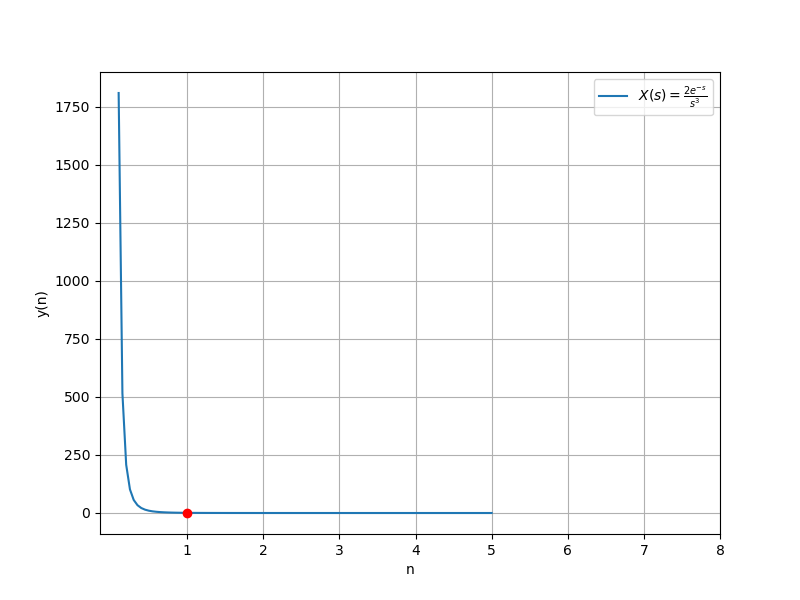
\includegraphics[width=\columnwidth]{figs/fig1.png}
  \caption{X(s) = $2e^{-s}/s^3$}
  \label{fig:graph}
\end{figure}
\end{document}
